%O+I
% Dominic feedback => final
% 23 Dec 2004

\ifx\wholebook\relax\else
\input{../Common.tex}
\input{../macroes.tex}
\begin{document}
\fi


\chapter{Directions and Angles}\label{ch:relativeTurn}


\begin{chapterfigure}
\hfil 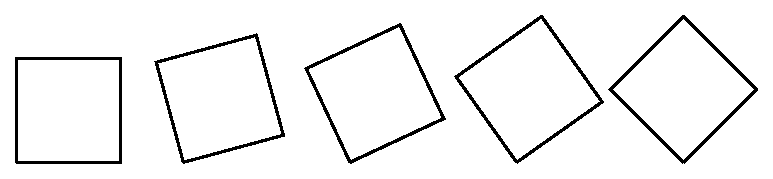
\includegraphics[width=0.9\linewidth]{ChTurntitlePicture}\hfil
\end{chapterfigure}


\hidden{
finalVersion
titlePicture
	
	| caro |
	caro := Turtle new.
	caro go: 50.
	caro turnLeft: 90.
	caro go: 50.
	caro turnLeft: 90.
	caro go: 50.
	caro turnLeft: 90.
	caro go: 50.
	caro turnLeft: 90.
	caro jump: 80.
	caro turnLeft: 15.
	caro go: 50.
	caro turnLeft: 90.
	caro go: 50.
	caro turnLeft: 90.
	caro go: 50.
	caro turnLeft: 90.
	caro go: 50.
	caro turnLeft: 90.
	caro east.
	caro jump: 80.
	caro turnLeft: 25.
	caro go: 50.
	caro turnLeft: 90.
	caro go: 50.
	caro turnLeft: 90.
	caro go: 50.
	caro turnLeft: 90.
	caro go: 50.
	caro turnLeft: 90.
	caro east.
	caro jump: 80.
	caro turnLeft: 35.
	caro go: 50.
	caro turnLeft: 90.
	caro go: 50.
	caro turnLeft: 90.
	caro go: 50.
	caro turnLeft: 90.
	caro go: 50.
	caro turnLeft: 90.
	caro east.
	caro jump: 80.
	caro turnLeft: 45.
	caro go: 50.
	caro turnLeft: 90.
	caro go: 50.
	caro turnLeft: 90.
	caro go: 50.
	caro turnLeft: 90.
	caro go: 50.
	caro turnLeft: 90
}

By now you should be getting tired of drawing figures only in \emph{fixed} directions. In this chapter you shall learn how to change the direction in  which a robot moves and draws a line in \emph{any} direction and in relative manner. For this purpose, we present the mathematical concept of angle to indicate to a robot how far it should turn. However, if you understand clearly what an angle is and how to measure angles in degrees, you may skip Section~\ref{sec:angles} and proceed readily with the examples and experiences of Section~\ref{sec:angleExperiments}. 

We start by presenting the elementary messages that robots understand to change their direction. Note that we are hiding the robots from the illustrations using the message \ct{beInvisible} so that you can get clearer pictures. 


\section{Right or Left?}\label{rightleft}
In the previous chapter, you learned that a robot could face different directions using the messages \ct{east}, \ct{north}, \ct{northEast}, \ct{northWest}, \ct{south}, \ct{southEast}, \ct{southWest} and \ct{west}. However, with these messages you can not change the direction of your robot from a given angle such as 15 degrees. In addition, you cannot say that you want for example turn a robot of a quarter of a turn from the current direction. 

To orientate a robot along any direction you should use the two methods
\turnLeft and \turnRight which ask a robot to turn to the left or the right. As the colon at the end of the names indicates, both methods are expecting an argument. This argument is the angle between the heading of the robot before and after issuing the message. This angle is given in degrees. For example the expression \ct{\caro turnLeft: 15} asks \caro to turn on the left fifteen degrees from its current direction and \ct{\caro turnRight: 30} turns on the right 30 degrees from its current direction. Figure~\ref{fig:turnLeftBoth} illustrates the effect of the messages \ct{turnLeft:} and \ct{turnRight:} first when a robot is pointing to the east and second when a robot is pointing to another direction.  


Now you should practice but remember that when a new robot is created, it always points to the east or the right of the screen. 

\begin{figure}
\begin{center}\includegraphics[width=16cm]{turnLeftBoth}
\caption{Left: turning left or right from the east position. Right: turning left of right from another position. \label{fig:turnLeftBoth}}
\end{center}
\end{figure}


\begin{exonofig} 
Read the following scripts Problem One (\scriptref{scr:proone}) and Problem Two (\scriptref{scr:protwo}) and try to guess what the created robot will do. Then experiment with the scripts: Change the angle values for example to determine what is the angle so that the robot turns a quarter, an half of a complete turn or a complete turn. If you have problem with the notion of angle read carefully the Section~\ref{sec:angles} before continuing.
\end{exonofig}


\begin{ncscript}{Problem One}\label{scr:proone}
| \caro |
\caro :=  \Turtle new. 
\caro go: 100.
\caro turnLeft: 45.
\caro go: 50.
\caro turnLeft: 45.
\caro go: 100\end{ncscript}

\begin{ncscript}{Problem Two}\label{scr:protwo}
| \caro |
\caro := \Turtle new. 
\caro go: 100.
\caro turnRight: 60.
\caro go: 100.
\caro turnLeft: 60.
\caro go: 100\end{ncscript}

\paragraph{About Mathematical Conventions.} In mathematics, there exist some conventions for the rotations: a rotation with a negative angle is clockwise and with a positive angle inverse clockwise. In this book, you can  also follow the mathematical conventions, using the message \ct{turn:}. Hence, the message \ct{turnLeft: anAngle} is equal to the message \ct{turn: anAngle} while, the message \ct{turnRight: anAngle} is equal to \ct{turn: - anAngle} that is the angle negated as shown by the Figure~\ref{fig:turnLeftWithMathematicalEq}. 


\begin{figure}
\begin{center}\includegraphics[width=8cm]{turnLeftWithMathematicalEq}
\caption{Some angles starting from the east directions.\label{fig:turnLeftWithMathematicalEq}}
\end{center}
\end{figure}




\section{Absolute versus Relative Orientation}
Now you should feel confident that you can ask a robot to execute any
drawing made with lines of any sort. Before going further, have you
understood the difference between orienting a robot using the
methods \north, \south, \east, and \west and using the methods \turnLeft and \turnRight?
Figure~\ref{fig:roserelative} shows some angles which are measured starting from the east direction. 

To explain the difference we ask you to complete the following experiments \ref{exo:relativeSquare}, \ref{expturntt} and \ref{expturntttwo}.

\begin{exofigwithsizeandtitle}[0.4]{\includegraphics[width=4cm]{ChTurnfirstSquare}}{A Relative Square} \label{exo:relativeSquare} 

\hidden{%%firstSquare
| caro |
	caro := Turtle new.
	caro go: 100.
	caro turnLeft: 90.
	caro go: 100.
	caro turnLeft: 90.
	caro go: 100.
	caro turnLeft: 90.
	caro go: 100.
	caro turnLeft: 90.}

Define a script drawing a square using the methods \turnLeft or \turnRight.
\end{exofigwithsizeandtitle}

\begin{exonofig}\label{expturntt}
Now, add the following line: \ct{\caro turnLeft: 33.}  before the first
line containing a \go message in the script you just defined.  As you can see one still obtains a square, but it is tilted. 
\end{exonofig}

\begin{exonofig}\label{expturntttwo}
Finally type the \scriptref{scr:badSquare} that draws a square but only using the methods \north, \south, \east and \west that we presented in the previous chapter. 
\end{exonofig}

\begin{scriptfigwithsize}{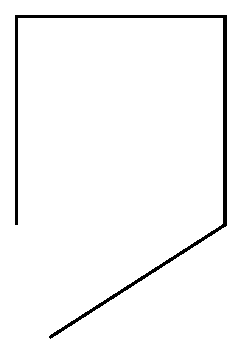
\includegraphics[width=4cm]{ChTurnbadSquare}}{A Broken Square} \label{scr:badSquare}
| \caro |
\caro := \Turtle new.
\textit{\caro \turnLeft 33.}
\caro go: 100.
\caro north.
\caro go: 100.
\caro west.
\caro go: 100.
\caro south.
\caro go: 100.
\end{scriptfigwithsize}

Do you still obtain a square? No! The first side drawn by the robot
is slanted whereas the other sides are either horizontal or
vertical. What these two scripts \scriptref{scr:badSquare} and
\scriptref{exo:relativeSquare} show you is the difference between
\emph{relative} and \emph{absolute} direction changes.

\begin{itemize}
\item The methods \north, \south, \east and \west change direction in an  \emph{absolute} manner.  The direction to which the robot will point does \emph{not} depend on the current direction in which it is pointing.

\item The methods \turnLeft and \turnRight change direction in a \emph{relative} manner. The direction to which the robot will point \emph{depends} on its current direction.
\end{itemize}

Figure~\ref{fig:roserelative} shows the equivalence between relative moves starting with a robot pointing to the east and absolute moves. As you know know, this equivalence is not correct if the robot is pointing to any other direction than the east. It is worth to note that turning 180 degrees makes the robot pointing in the opposite direction which is often used in the scripts.

\begin{figure}[h]
\begin{center}\includegraphics[width=8cm]{roseDesVentsRelatifToo}
\caption{Comparing absolutes and relative angles starting from the east direction.\label{fig:roserelative}}
\end{center}
\end{figure}


\section{The Right Angle of Things}\label{sec:angles}
As you should know by now, a newly created robot is pointing east,
that is, toward the right hand side of the screen. If we ask this
robot to turn left by 90 degrees, it will end up heading north. If we
ask it to turn right by 90 degrees, it will end up heading south. Here
is a script (\ref{scr:angleSearch}) illustrating what a turn left by 45 degrees is doing. To help you following it we added the starting position of the robot.

\begin{scriptfig}{ChTurnangleSearchAnnotated}{The meaning of angles} \label{scr:angleSearch}
| \caro |
\caro := \Turtle new.
\caro west.
\caro go: 100.
\caro east.
\caro turnLeft: 45.
\caro go: 100.
\end{scriptfig}

The first part of script~\ref{scr:angleSearch}, up to the line \ct{\caro east}, draws an
horizontal line to indicate the eastern direction. The last part draws
the line in the direction 45 degrees left of the east direction. You
can vary the value of the angle to see what other values
represent. Try the values 60, 120, 180, 240, 360, and 420. In
particular, note that a turn by 180 degrees amounts to going back on the
previous direction.

Do you see any difference between 60 and 420? No. Any two angle values
whose difference is 360 or any multiple thereof are equivalent. Try an
angle value of  1860 ($1860 = 60  + 360 \times 5$). The  result is the
same as  that with angle values  60 and 420.  360  degrees represents a
single turn. As  far as orienting oneself, it  does not matter whether
you add one  or more full turns to the orientation.  Keep this in mind
when dealing with angles.

Now, let us try the method \turnRight. Script~\ref{scr:angleSearch2} draw two needles of and old watch and a reference line. It uses two robots, that you can use to investigate the correspondence between a left or a right turn.  We added comments surrounded by \ct{"} and use different font effects to help you to identify the different parts in the script. Note that you do not have to type these comments as they do not get executed. 


%%DoubleTurtles@@
\begin{scriptfig}{twoAnglesAnnotated}{The meaning of angles (2)} \label{scr:angleSearch2}
| \caro daly |
\caro := \Turtle new.
\emph{\caro jump: 200.}                        "drawing the reference line"
\emph{\caro turnLeft: 180.
\caro go: 200.
\caro turnLeft: 180.}
\caro color: Color blue.
\caro turnLeft: 45.                 "drawing the long needle"
\caro go: 150.
daly := \Turtle new.
daly color: Color red.
\textbf{daly turnRight: 45.}              "drawing the short needle"
\textbf{daly go: 100.}                             
\end{scriptfig}

In script~\ref{scr:angleSearch2}, the code in italic draws the reference line --- that is the line representing the direction of the robot before issuing a turn method
--- using the fact that a turn by 180 degrees amounts to go back in the
opposite direction. The reference line is also the  longest lines drawn. Thus, 
the reference line will still be visible if the lines drawn by the robots fall on top of it. 
Then in normal font is the code that draws the longest needle (using \caro) and in bold the code drawing the short needle using the variable \ct{pica}. This is similar to the needles of an old time clock.

%The reference line, that is the line representing the initial direction, is drawn by \caro, but it is common to both robots. Indeed, we have seen that all robots are created equal.  In particular, they both point to the eastern direction initially.

\begin{exonofig} Repeat the same series of angle values for both
 robots, that is, change the angle value for the two turn methods.
Then, compare the effect of the method \turnLeft\ \ct{60} (for
\caro) and \turnRight\ \ct{300} (for {\ct{daly}}). You can see
that turning left by 60 degrees is the same as turning right 300
degrees because the sum of the two values is 360 degrees, that is a
full turn.
\end{exonofig}

\begin{exonofig} 
Now let us see what happens when turning from another direction.  Here
is the same script as \scriptref{scr:angleSearch} but showing the
effect of turning from the north direction.

%%DoubleTurtles@@
\begin{scriptfig}{threeAngles}{The meaning of angles (3)} 
\label{scr:angleSearch3}
| \caro marge |
\caro := \Turtle new.
\textbf{\caro north.}
\caro jump: 200.
\caro turnLeft: 180.
\caro go: 200.
\caro turnLeft: 180.
\caro color: Color blue.
\caro turnLeft: 45.
\caro go: 150.
daly := \Turtle new.
daly north.
daly color: Color red.
daly turnRight: 45.
daly go: 100.
\end{scriptfig}
\end{exonofig} 

\begin{exonofig}
Continue to experiment with the \scriptref{scr:angleSearch3} by changing
the direction of reference. For the comparison to be meaningful, you
have also to orient \ct{daly} to the same direction than \caro after
creating it. Try any angle values you like and try to predict what the
resulting drawing will look like before executing the script. Continue
experimenting with that script until your predictions are good.
\end{exonofig}

Note that it is important that you can always predict what is going to happen
before executing a script because a computer blindly executes statements, even the silliest ones.


\section{A Robot Clock}
We have mentioned that the lines drawn in the \scriptref{scr:angleSearch3}
were akin to that of an old time watch. The analogy is more than
real. The notion of degrees is strongly correlated to that of hours,
because the ancient peoples discovered the notion of time by measuring the
angle of the sun (or some star) respective to a direction of reference.
However with the previous code you could draw a clock indicating an hour that was not true, that is the small needle pointing to the north and the long one to the south. 

Now you will study the relationship between the small needle and the long one to represent a \emph{real} hour: if the long needle is pointing on the south then the short one should be half of the hour distance between two numbers. Modify \scriptref{scr:angleSearch3} and proceed as follows:

\begin{enumerate}
\item Keep the direction of reference to the north (this is how
\scriptref{scr:angleSearch3} is written). The reference line
indicates noon.
  
\item Use the method \turnRight for both robots. A turn
 to the right is what the needles of an old time clock are doing.
  
\item You can ask \caro to draw the minute needle by
multiplying the number of the minutes you want to indicate by 6.
For example, 20 after the hour is shown with the message 
\ct{turnRight: 120} ($120 = 6 \times 20$).
  
\item You can ask \ct{marge} to draw the hour needle by
multiplying the number of the hours you want to indicate by 30.
For example, 2 o'clock is shown with the message
\ct{turnRight: 60} ($60 = 30 \times 2$).
\end{enumerate}

Try to indicate a few hours of your choice with that script.

\section{Simple Drawings}\label{sec:angleExperiments} 
To begin with, here is a script drawing a triangle:

\begin{scriptfigwithsize}[0.4]{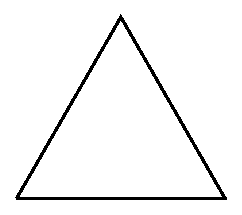
\includegraphics[width=4cm]{ChTurnfirstTriangle}}{A triangle} \label{scr:firstTriangle}
| \caro |
\caro := \Turtle new.
\caro go: 100.
\caro turnLeft: 120.
\caro go: 100.
\caro turnLeft: 120.
\caro go: 100
\end{scriptfigwithsize}

Now, you are ready to draw a house.

\begin{exofigwithsize}{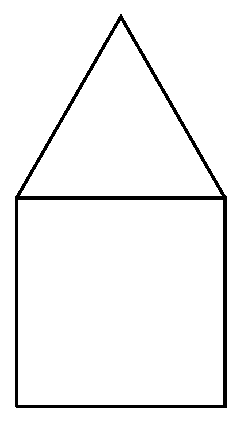
\includegraphics[width=2cm]{ChTurnbabyHouse}}\label{exo:babyHouse} 
Draw a house as shown on the right. Try to draw houses of different shapes.
\end{exofigwithsize}

\hidden{%%babyHouse
	| caro |
	caro := Turtle new.
	caro go: 100.
	caro turnLeft: 90.
	caro go: 100.
	caro turnLeft: 90.
	caro go: 100.
	caro turnLeft: 90.
	caro go: 100.
	caro turnLeft: 180.
	caro jump: 100.
	caro turnRight: 90.
	caro jump: 100. 
	caro turnLeft: 120.
	caro go: 100.
	caro turnLeft: 120.
	caro go: 100}



\section{Regular polygons} \label{sec:firstPolygons} 
A regular polygon is a figure made with line segments of the same
length. An equilateral triangle is a regular polygon with 3 sides. A
square is a regular polygon with 4 sides.  For example, the
\scriptref{scr:firstTriangle} that draws an equilateral triangle,
whose side length is 100 pixels, is obtained by asking \caro to go
forward a given distance and to turn 120 degrees left or right, the two
commands repeated 3 times. Note that there is a relationship between the 
number of sides and the angle: the angle is equal to 360 degrees divided 
by the number of sides. 

Program a robot to draw a regular polygon with any number of
sides by asking it to go for some length and then turn left or right
by 360 degrees divided by the number of sides; this sequence must be
repeated as many times as there are sides.




\begin{exofig}{ChTurnpentagon} \label{exo:pentagon}
Try to draw a pentagon, that is a regular polygon with five sides
of 100 pixel length.
\end{exofig}

\hidden{	| caro |
	caro := Turtle new.
	caro go: 100.
	caro turnLeft: 72.
	caro go: 100.
	caro turnLeft: 72.
	caro go: 100. 
	caro turnLeft: 72.
	caro go: 100.
	caro turnLeft: 72.
	caro go: 100.}

\begin{exofig}{ChTurnhexagon} \label{exo:hexagon}
Try to draw a hexagon, that is a regular polygon with six sides of
100 pixel length.
\end{exofig}

\hidden{%%Hexagon
	| caro |
	caro := Turtle new.
	caro go: 100.
	caro turnLeft: 60.
	caro go: 100.
	caro turnLeft: 60.
	caro go: 100. 
	caro turnLeft: 60.
	caro go: 100.
	caro turnLeft: 60.
	caro go: 100.
	caro turnLeft: 60.
	caro go: 100.}

Maybe, you are just curious to see how far you can go. Using the
cut and paste facility of the \tw, you can
actually generate a regular polygon with a large number of sides.
If you are in the mood, go on increasing the number of sides. However
in the next chapter we will show you how this can be solved. 

\ 


\begin{exofigwithsize}{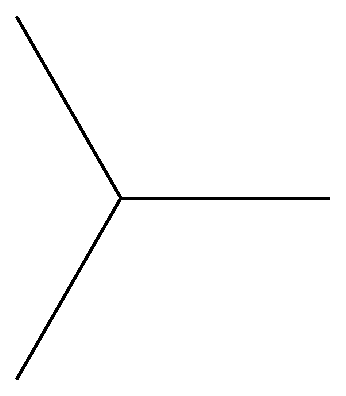
\includegraphics[width=4cm]{ChTurnc3pace}}\label{exo:pace}
Draw the symbol shows by the figure on the  right.
\end{exofigwithsize}



\hidden{c3pace
| caro |
	caro := Turtle new.
	caro go: 100.
	caro turnLeft: 180.
	caro jump: 100.

	caro turnLeft: 60.
	caro go: 100. 
	caro turnLeft: 180.
	caro jump: 100. 

	caro turnLeft: 60.
	caro go: 100. 
}


\summa
\begin{enumerate}
\item A robot can be oriented \emph{relatively} to its \emph{current}
  direction using the methods \turnLeft and \turnRight.
\item The parameter given to the methods  \turnLeft and
\turnRight is given in degrees.
  \item Turning 360 degrees corresponds to a full turn.
	\item Turning  180 degrees corresponds to an half turn.
  \item Angles values whose difference is a multiple of 360 degrees
  are equivalent.
\end{enumerate}

Here is the list of the methods which you have learned in this chapter.
\begin{table}[h]
  \centering
  \begin{tabular}{| l | p{5cm} | l |} \hline
  % after \\ : \hline or \cline{col1-col2} \cline{col3-col4} ...
  \hfil Method & \hfil Description & \hfil Example \\[1ex] \hline
  \turnLeft & Ask the robot to change its direction to a number of given degrees to the left & \ct{\caro turnLeft: 30} \\ \hline
   \turnRight & Ask the robot to change its direction to a number of given degrees to the right & \ct{\caro turnRight: 30} \\
  \hline
   \ct{turn:} & Ask the robot to change its direction to a number of given degrees following the mathematical convention:  to the left is the number is positive and to the right if it is negative & \ct{\caro turn: -30} \\ \hline

\ct{beInvisible}& Hide the receiver & \ct{\caro beInvisible} \\
  \hline
\ct{beVisible}&Show the receiver& \ct{\caro beVisible} \\
  \hline

\end{tabular}
\end{table}


\ifx\wholebook\relax\else\end{document}\fi
